\chapter{Asim: approximate analytical simulation}
\label{chap:asim}

\begin{figure}
% \hrule
\vspace{1em}
\centerline{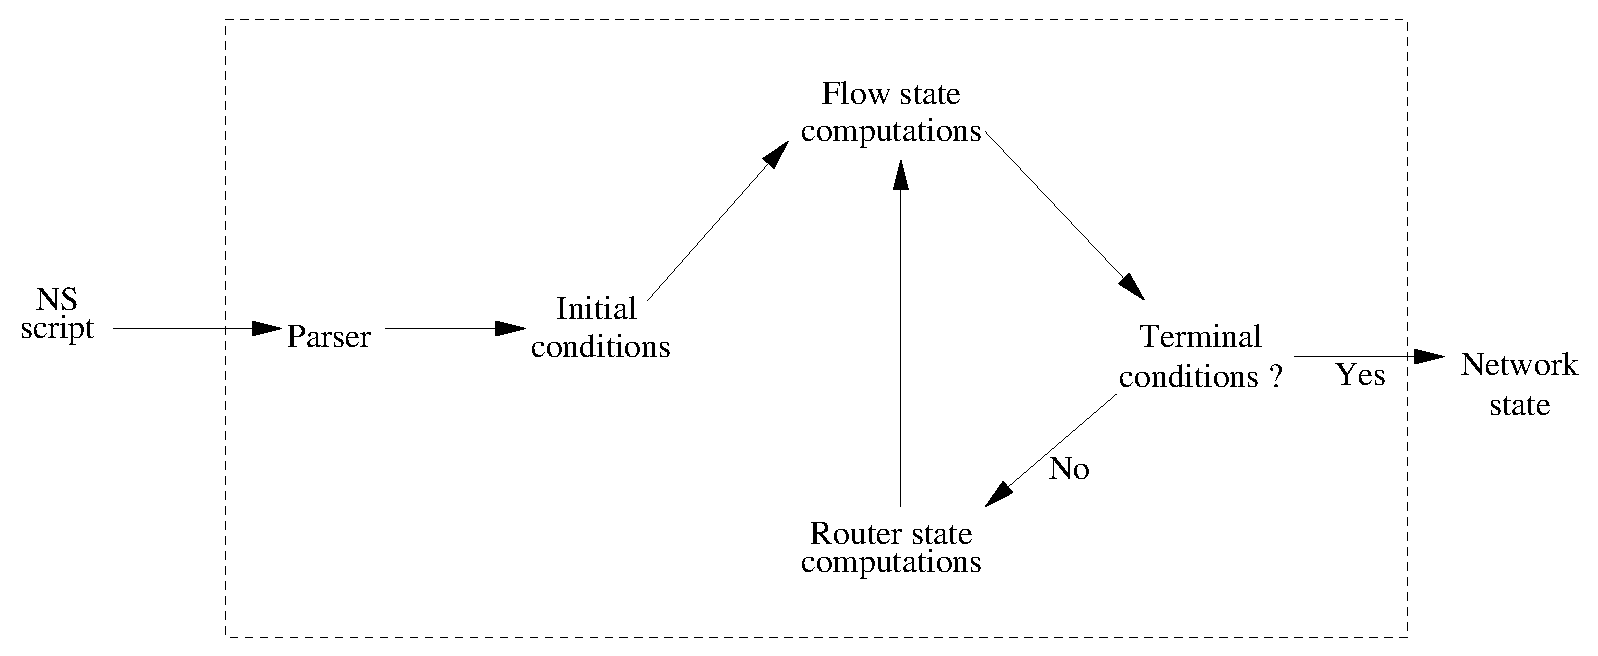
\includegraphics[angle=0,width=5in]{figures/struct.eps}}
\vspace{1em}
% \hrule
\caption{The structure of Asim}
\label{fig:struct}
\end{figure}


This chapter describes a fast approximate network simulator, Asim. 
Asim solves the steady state of the network using 
approximate fixed points. The overall structure is shown in 
Figure \ref{fig:struct}.
The user feeds a regular ns script 
and turns on the asim flag.
Asim would do a fast approximate simulation of the 
network scenario and would present to the user the drop probabilities
of the routers, 
the delays and the approximate aggregate throughput 
of the links and the flows.

In particular, we the following links/traffic are supported:
\begin{itemize}
\item Drop Tail Queues
\item RED Queues
\item Bulk TCP flows with FTP traffic
\item Short lived TCP flows 
\end{itemize} 

The data structures of Asim 
are populated by a module within the Tcl space of ns from the 
user supplied script. Upon executing Asim, the results can 
be accessed using Tcl routines. 
To use the Asim within a script the user has to use 

\noindent Simulator set useasim\_ 1

\noindent By default, this flag is set to 0

A simple script is given below

\begin{verbatim}

proc addsrc { s } {
    global ns
    set t [$ns set src_]
    lappend t $s
    $ns set src_ $t
}

proc adddst { src } {
    global ns
    set t [$ns set dst_]
    lappend t $src
    $ns set dst_ $t
}




proc finish {} {
    
    global ns fmon

    set drops  [$fmon set pdrops_]
    set pkts   [$fmon set parrivals_]
    set notDroped [$fmon set pdepartures_]

    set overflow_prob [expr 1.0 * $drops / $pkts]
    puts [format "tdrops $drops tpkts $pkts o_prob. %7.4f" $overflow_prob]

    exit 0

}

set N_ 100000
set arrival 0
set available $N_
set endTime_ 200

set ns [new Simulator]
$ns set useasim_ 1
$ns at $endTime_ "finish"

set src_ ""
set dst_ ""

$ns set src_ $src_
$ns set dst_ $dst_

set n(0) [$ns node]
set n(1) [$ns node]
set link(0:1) [$ns duplex-link $n(0) $n(1)  1Mbps  50ms RED]

for {set i 0} { $i < 4} {incr i} {

	set ltcp($i) [new Agent/TCP]
	set ltcpsink($i) [new Agent/TCPSink]
	$ns attach-agent $n(0) $ltcp($i)
	$ns attach-agent $n(1) $ltcpsink($i)
	$ns connect  $ltcp($i) $ltcpsink($i)

	set lftp($i) [new Application/FTP]
	$lftp($i) attach-agent $ltcp($i)
	$ns at 0 "$lftp($i) start"

}

# Short term flows
addsrc 1
adddst 0

set pool [new PagePool/WebTraf]

# Set up server and client nodes
$pool set-num-client [llength [$ns set src_]]
$pool set-num-server [llength [$ns set dst_]]
global n
set i 0
foreach s [$ns set src_] {
        $pool set-client $i $n($s)
        incr i
}
set i 0
foreach s [$ns set dst_] {
        $pool set-server $i $n($s)
        incr i
}

# Number of Pages per Session
set numPage 100000

$pool set-num-session 1

set interPage [new RandomVariable/Exponential]
$interPage set avg_ 0.5

set pageSize [new RandomVariable/Constant]
$pageSize set val_ 1

set interObj [new RandomVariable/Exponential]
$interObj set avg_ 1

set objSize [new RandomVariable/Constant]
$objSize set val_ 20

# This is needed
$pool use-asim

$pool create-session 0 $numPage 0 $interPage $pageSize $interObj $objSize

# Dumps internal data structures to this dumpfile
$ns asim-dump dumpfile

# Calls asim-run 
$ns asim-run

# Access asim statistics
set l [$ns link $n(0) $n(1)]
puts "after asim run, link bw = [$ns asim-getLinkTput $l] packets"
puts "after asim run, flow bw = [$ns asim-getFlowTput $ltcp(0)] packets"

\end{verbatim}









